\section{Requirements} \label{sec:Requirements}

Benett et al. (2010,p. 140-142) \nocite{bennett2010object} categorises
requirements as of three types:

\begin{description} \item[Functional Requirements]
    The system's functionality -- what it is expected to do.
    
  \item[Non-functional Requirements]
    How well the system delivers its functionality. These requirements are
    related to the performance, scalability, availability, recovery time,
    security, and others.

  \item[Usability Requirements]
    These relate to how effectively, efficiently and satisfactorily users can
    achieve their goals in the existing system. User interfaces can play a big
    part in meeting these requirements.
\end{description}

The initial implementation iterations will be focused more on the functional
and usability requirements, paying some attention as well to specific
non-functional requirements such as performance and security.


\subsection{Functional Requirements} \label{sec:Requirements.FunctionalRequirements}


Use case diagrams are an UML construct which were developed by Jacobson et al.
(1992, cited \cite[][p.~154]{bennett2010object}). The use case diagram below is
used to illustrate the functional requirements listed above:

\begin{figure}[ht!]
  \begin{center}
    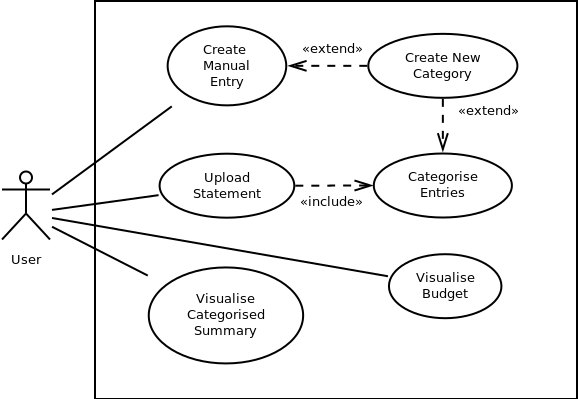
\includegraphics[width=14cm]{./contents/img/Use_Case_Diagram.png}
  \end{center}
\end{figure}
\FloatBarrier
